\section{Auswertung}
\label{sec:Auswertung}
In diesem Abschnitt werden die Messdaten ausgewertet, um die Bragg Bedingung zu überprüfen, um das Emissionspektrum der Kupferröhre zu bestimmten und um die Absorptionsspektren von Brom, Gallium, Rubidium, Strontium und Zink zu bestimmen.
\subsection{Bragg}
Für die Überprüfung der Bragg Bedingung wurden die in \autoref{fig:bragg1} aufgelisteten Daten verwendet.
\begin{figure}[H]
  \centering
  \includegraphics{daten/bragg.JPG}
  \caption{Bragg Daten}
  \label{fig:bragg1}
\end{figure}
In \autoref{fig:bragg2} wurden die pro Sekunde aufgenommenen Impulse in Abhänigkeit des Winkels dargestellt. Das gesuchte Maximum ist farblich markiert.
\begin{figure}[H]
  \centering
  \includegraphics{build/bragg.pdf}
  \caption{Impulse pro Sekunde in Abhängigkeit des Winkels zur Überprüfung der Bragg Bedingung}
  \label{fig:bragg2}
\end{figure}
\noindent
Das Maximum der Messdaten liegt bei $N=218 Imp/s$ mit dem Winkel $\theta=28,2°$. Der theoretische Glanzwinkel für die Anordnung mit dem LiF-Kristall beträgt $28°$. Die Abweichung des Messwertes vom Theoriewert beträgt somit $\Delta \theta=0,2°$ bzw. $\Delta \theta_{rel}=0,72\%$.
\subsection{Emissionsspektrum}
In \autoref{fig:spektrum} sind die Messdaten zum Emissionsspektrum der genutzten Kupferröhre dargestellt. Dazu sind die $K_\alpha-$ und $K_\beta-$Linie zu sehen, die bei
\begin{align*}
    \theta_{K_\alpha} &= \SI{22.5}{\degree} \\
    \theta_{K_\beta}  &= \SI{20.2}{\degree} \; 
\end{align*}
liegen.
\begin{figure}[H]
  \centering
  \includegraphics{build/spektrum.pdf}
  \caption{Emissionsspektrum der genutzten Kupferröhre, dargestellt sind die Messdaten, die $K_\alpha-$ und die $K_\beta-$Linie.}
  \label{fig:spektrum}
\end{figure}
\noindent
Mit den im Theorie-Teil erläuterten Formeln lassen sich $\text{E}_\text{max}, \lambda_\text{min}$ und $\theta_\text{Grenz}$ wie folgend berechnen($U=35 \si{\kilo\volt}$):
\begin{align*}
  \text{E}_\text{max} &= 35 \, \mathrm{keV}\\
  \lambda_\text{min} &= 354.241 \, \mathrm{nm}\\
  \theta_\text{Grenz} &= 5.045°
\end{align*}
Für die $K_\alpha-$ und die $K_\beta-$Linie ergeben sich:
\begin{align*}
  \theta_\alpha&=20.2° & \theta_\beta&=22.5° \\
  \text{E}_\alpha&=8.0434 \, \mathrm{keV}   &\text{E}_\beta&=8.9142 \, \mathrm{keV} \\
  \Delta\text{E}_{\text{FWHM}\alpha}&=165.63 \, \mathrm{V}   &\Delta\text{E}_{\text{FWHM}\beta}&=205.58 \, \mathrm{V} \\
  \text{A}_\alpha&=48.56  &\text{A}_\beta&=43.36 \\
  \end{align*}
\subsection{Absorptionsspektren}
Im Folgenden werden die Absorptionsspektren 5 verschiedener Absorber untersucht. In \autoref{fig:Brom} bis \autoref{fig:Zink} sind die gemessenen Zählraten pro Sekunde $N$ in Abhängigkeit der Winkel $\theta$ für Brom, Gallium, Rubidium, Strontium und Zink dargestellt. 
\begin{figure}[H]
  \centering
  \includegraphics{build/Brom.pdf}
  \caption{Brom}
  \label{fig:Brom}
\end{figure}

\begin{figure}[H]
  \centering
  \includegraphics{build/Gallium.pdf}
  \caption{Gallium}
  \label{fig:Gallium}
\end{figure}

\begin{figure}[H]
  \centering
  \includegraphics{build/Rubidium.pdf}
  \caption{Rubidium}
  \label{fig:Rubidium}
\end{figure}

\begin{figure}[H]
  \centering
  \includegraphics{build/Strontium.pdf}
  \caption{Strontium}
  \label{fig:Strontium}
\end{figure}

\begin{figure}[H]
  \centering
  \includegraphics{build/Zink.pdf}
  \caption{Zink}
  \label{fig:Zink}
\end{figure}